\documentclass[
	11pt, 
	DIV10,
	ngerman,
	a4paper, 
	oneside, 
	headings=normal, 
	captions=tableheading,
	final, 
	numbers=noenddot
]{scrartcl}


\usepackage[ruled]{algorithm2e}
\usepackage{graphicx}
\usepackage{hyperref}
\usepackage{amsmath}


\title{Fully Asynchronous SPH Simulation}
\subtitle{\vspace{0.5cm}Seminar: Current Topics in Fluid Animation}
\author{Yinglun Liu}


\begin{document}
\maketitle


\section{Motivation}

Over the years, the adoption of smoothed particle hydrodynamics(SPH) has developed to become the common pratice when simulating fluids in various scenes. In non-iterative approaches, the physical state of a fluid particle is constantly influenced by its immediate neighborhood and is thus updated in each time step following a few governing equations that enforces the incompressibility of the fluid. In these equations, the computation of new attributes of the current particle requires several times the access to information from its surrounding neighbors. Intuitively, a natural practice would be to, as did many non-iterative SPH solvers, perform global updates to all particles using a single uniform time step. While iterative SPH solvers nowadays generally yield better performances, traditional non-iterative approaches do not seem to lessen in popularity due to the fact that they are easy to implement and suitable for less turbulent fluids.
\par
Be that as it may, a core defect of non-iterative SPH solvers may lie in the lack of efficiency. On one hand, to enforce a constantly negligible density deviation within the fluid, large stiffness parameters are adopted to generate high pressures. Such selection of parameters demands smaller time steps and, in turn, a greater number of iterations for stable and correct particle interations. This can lead to tremendously higher overhead for the generation of visually realistic animation, where tens of millions of particles are included to allow for as fine-grained details as possible. On the other hand, the author made the observation that, while smaller time steps are essential in heavily interacting regions to guarantee stable simulation, in many less complex parts of the fluid a larger time step suffices (see fig. \ref{fig:1}). That is, the maximum possible time step for a particle varies substantially across different regions of the simulation, and it makes less sense to set one global time step for all particles, since it would inevitably be limited by the single particle with the strictest time constraint and lead to much waste of computational power.

\begin{figure}[tb]
	\centering
	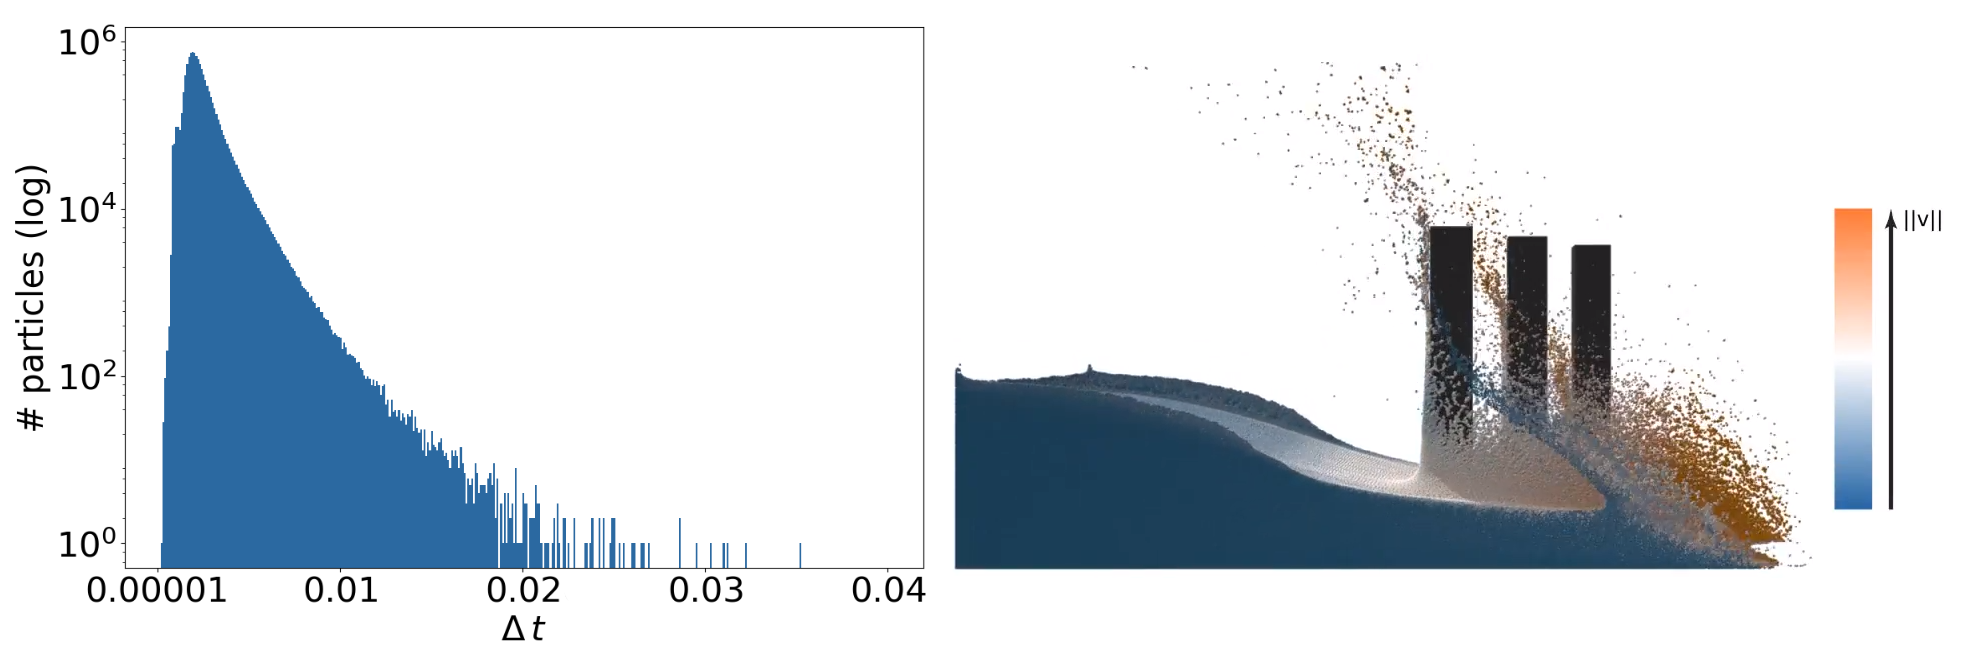
\includegraphics[scale=0.3]{images/1}
	\caption{
		\label{fig:1} For fluid simulation based on SPH, the magnitude of velocity differs substantially 			across particles from different regions (right). As a result, the maximum possible time steps for each 		individual particle could diverge to cover up to multiple magnitudes (left) \cite{reinhardt2017fully}.
	}
\end{figure}

\par
To cope with this, the author proposes a novel method for the time integration of particles, in which each particle is assigned a individual time step and the whole simulation is carried out fully asynchronous. To ensure consistency, the neighborhood is reconstructed at the current time stamp each time a particle is processed. To demonstrate the strength of the proposed method, the author further proposes a multi-queue parallelization to such fully asynchronous integration procedure. Comparative experiments against related works were conducted under diverse conditions and environments to prove the efficacious enhancement on performance.

\section{Related Work}

\section{Non-iterative SPH}

Governed by the Navier-Stokes equation \ref{equa:1}, non-iterative SPH performs interpolation over the neighborhood of a particle to calculate its attributes and ultimately the forces it incurs within one time step of the simulation. The fluid attribute $ A(x_{i}) $ of particle i at position $ x_{i} $ is computed as the weighted sum of  $ A(x_{j}) $ over all neighboring particles j, with the weights given by a normalizing kernel function W that is of compact support. After all forces are computed, time integration methods like symplectic euler or leap frog is carried out to update particle position and speed.

\begin{equation}
	\label{equa:1}
	\frac{\delta v}{\delta t} = -\frac{\nabla p}{\rho} + \nu v^{2} + \frac{F^{external}}{\rho}
\end{equation}

\subsection{Split Equations of State}

The author adopts here the splitting strategy as described by \cite{ihmsen2014sph}, where for each update step the advection forces $ F^{advection} $ are separately computed and then used to calculate an intermediate advection velocity $ v^{*} $. An advection density $ \rho^{*} $ is introduced to represent the expected density at the end of this time step as a result of the divergence in the velocity field if no compensating pressure force is generated. pressures $ p $ pressure forces $ F^{pressure} $ are afterwards handled conventionally. This updating scheme forces the solver to implicitly consider the impact of advection forces before generating pressure forces to counteract the deviation of density and therefore stablizes the simulation.

\vskip 0.2in
\begin{algorithm}[H]
	\caption{one global step with splitting \cite{reinhardt2017fully}}
	\label{alg1}
	\DontPrintSemicolon
	\SetAlgoLined
	\SetKwFunction{FMain}{Main}
	\SetKwProg{Fn}{Function}{:}{}
	\Fn{\FMain{}}{
		\For{each particle i}{
			find neighbors j\;
		}
		\For{each particle i}{
			compute advection force $ F_{i}^{*} = F_{i}^{viscosity} + F_{i}^{ext} $\;
			compute advection velocity $ v_{i}^{*} $ using $ F_{i}^{*} $\;
		}
		\For{each particle i}{
			compute advection density $ \rho_{i}^{*} $\;
			compute pressure $ p_{i} $\;
		}
		\For{each particle i}{
			compute pressure force $ F_{i}^{*} $\;
			compute new particle velocity $ v_{i}(t + \delta t) $\;
			compute new particle position $ x_{i}(t + \delta t) $\;
		}
	}
\end{algorithm}
\vskip 0.2in

Conventionally, a single global update step with the concept of spitting applied proceeds as in alg. \ref{alg1}. To interpolate particle properties a neighborhood search is conducted at each time step to fetch the set of neighbors for each particle. Since such operations can be computationally expensive, spatial data
structures(e.g. a uniform grid) that supports parallel operations are usually constructed at the beginning to accelerate the process. At each global step, the grid cells are queried and updated to efficiently maintain neighborhood information. To further minimize time consumed by inevitable query operations at each time step, particles are sorted in accordance with their spatial cell. In this fashion, spatially adjacent particles are stored on adjacent memory slots, enhancing the cache-hit rates during the simulation. Here, the author choose Z-index curve, a commonly used sorting function that effectively preserves spatial locality due to its fractal block structure.
\par
The advection force incurred by a particle consists of a viscosity component and some external components. The second order spatial derivative of velocity reflects the diverging trend of the local velocity field and decides the viscosity component. But since second order derivatives are tricky to compute, the approximation form proposed originally by \cite{monaghan1992smoothed} is prefered instead. Therefore the viscosity component acting on particle i is computed as

\begin{equation}
	\label{equa:2}
	F_{i}^{viscosity} = 2m_{i}\nu \sum_{j}\frac{m_{j}}{\rho_{j}}v_{ij}\frac{x_{ij} \cdot \nabla W_{ij}}{x_{ij}\cdot x_{ij} + 0.01h^{2}}
\end{equation}

where $ \nu $ is a hyperparameter describing the viscocity of the liquid. Since modeling boundary interations and surface tension is not a core theme of this paper, the author directly adopts the method of \cite{akinci2012versatile} and \cite{huber2015evaluation} to handle these two aspects of the advection force.
\par
Based on the advection forces, intermediate advection velocity is computed as follows:

\begin{equation}
	\label{equa:3}
	v_{i}^{*} = v_{i}(t) + \delta t\frac{F_{i}^{advection}}{m_{i}}
\end{equation}

This equation can be perceived as an intermediate velocity update using symplectic Euler without considering the impact of pressure forces. The first order spatial derivative of velocity reflects the divergence of the velocity field and is used to compute the advection density. Again, the author chooses the robust variant presented by \cite{monaghan1992smoothed} and computes the advection density via

\begin{equation}
	\label{equa:4}
	\rho_{i}^{*} = \sum_{j}m_{j}W_{ij} + \delta t_{i}\sum_{j}(v_{i}^{*} - v_{j}^{*})\cdot \nabla W_{ij}
\end{equation}

where the first term describes the static density at particle position $ x_{i} $ and the second term describes the density change during step $ \delta t_{i} $ as a consequence of diverging velocity field.
\par
Having obtained the advection densities of the particles, pressure at particle position $ x_{i} $ is computed as $ p_{i} = k(\rho_{i}^{*} - \rho_{0}) $, where $ \rho_{0} $ is the system's reference density and k is the stiffness parameter. Negative pressures are clamped to zero as in \cite{ihmsen2013implicit} to prevent the water splashes from being absorbed as a result of the induced cohesive effect. Finally, the respective pressure forces are calculated using the momentum-preserving variant:

\begin{equation}
	\label{equa:5}
	F_{i}^{pressure} = -m_{i}\sum_{j}m_{j}(\frac{p_{i}}{(\rho_{i}^{*})^{2}} + \frac{p_{j}}{(\rho_{j}^{*})^{2}})\nabla W_{ij}
\end{equation}

This pressure force is then solely responsible for the explicit velocity and position update of the particle, which we discuss in the next subsection.

\subsection{Time Integration}

\section{Method}

\section{Experiments}

\section{Conclusion}

\bibliographystyle{alpha}
\bibliography{references}

\end{document}          
